% !TeX root = ../thesis.tex

\chapter{Experimental Setup}
\label{sec:experimentatl_setup}


This chapter aims to define network architecture implementation details as well as experimental setup for panoptic segmentation architecture. Furthermore, it defines specifications for hyper-parameters. Hyper-parameter manipulation among
the experiments is kept to a minimum to ensure comparability and meaningful evaluation of the results.


\section{Network Architecture}


Typical approaches for instance and semantic segmentation have diverged in literature and each task usually
adopts fundamentally different kind of network architecture. There has not been many approaches that deal with both segmentation modalities following a similar approach. However, panoptic segmentation has been introduced as a unified segmentation task \cite{DBLP_panootic_seg:journals/corr/abs-1801-00868} which demands to tackle panoptic segmentation task within a single network architecture. To this end a unified network architecture has been implemented. 


Panoptic segmentation architecture implemented during the course of this master thesis relies on feature extractor based on a modern semantic segmentation architecture called \textit{DeepLab} \cite{Deeplabv3+:journals/corr/abs-1802-02611}. This semantic segmentation architecture has an encoder-decoder structure as shown in figure \ref{fig: deeplab_diag} that helps in gradually recovering spatial resolution and results in better recovered boundaries between different semantic classes. Deeplab also uses a combination of \textit{depth-wise separable convolutions } and \textit{atrous convolutions} as shown in \ref{fig:Depthwise_sep_conv} and \ref{fig:atrousconv} respectively. A depth-wise separable convolution that uses atrous convolutions i.e. convolution filters with padded zeros between learnable kernel values is called \textit{atrous separable convolutions} which has been explained in section \ref{subsec:atroussepconv}. Additionally, it employs a special kind of pooling module that applies multiple parallel atrous convolutions at different rates and concatenates them to collect the features from an input feature map, which is equivalent to pooling features at multiple spatial resolutions, hence equivalent to a \textit{feature pyramid}. This pooling module has been called \textit{Atrous Spatial Pyramid Pooling Module} (ASPP) and is augmented at the latent space of encoder. Owing to the above mentioned modules, deeplab is considered to be one of the sophisticated semantic segmentation architecture that utilizes efficient convolution operations, with dense feature extracting modules and encoder-decoder structure that aids semantic segmentation like tasks. A typical deeplab architecture has been shown in the figure \ref{fig: deeplab_diag}. 



\begin{figure}[!ht]
%\centering
\subfigure[Depth-wise Separable Convolution]{
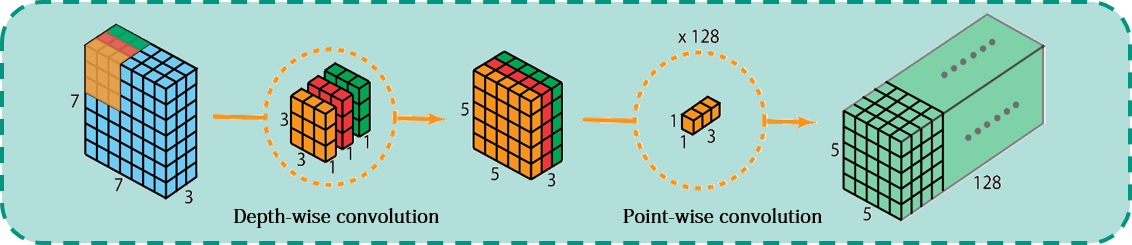
\includegraphics[width = \textwidth ]{Graphics/Experimental_Setup/Depthwise Seperable Convolution}
\label{fig:Depthwise_sep_conv}}

\subfigure[Atrous Convolutions]{
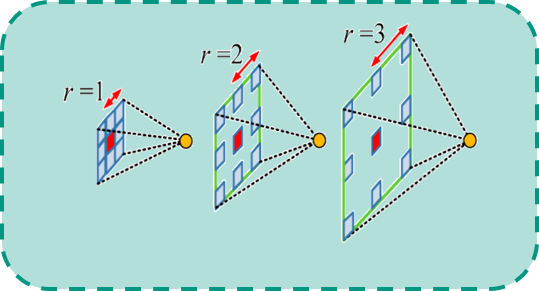
\includegraphics[width = \textwidth / 2 ]{Graphics/Experimental_Setup/atrous_conv}
\label{fig:atrousconv}}
\subfigure[Atrous Spatial Pyramid Pooling]{
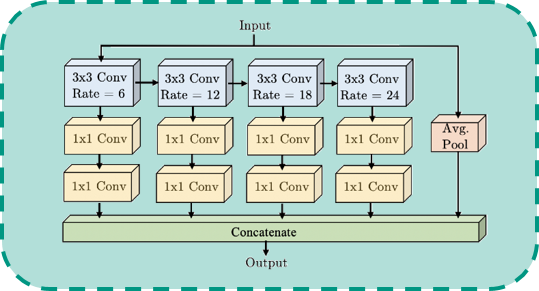
\includegraphics[width = \textwidth / 2 ]{Graphics/Experimental_Setup/atrous_spatial_pyramid_pooling}
\label{fig:aspp}}
\caption[Features of Deeplab ] {Illustration of some interesting features from DeepLab a) shows an illustration of a depth-wise separable convolution - a combination of depth-wise convolution followed by a point-wise convolution \cite{DEPSEPCONV} b) shows atrous convolutions - where zeros are padded in between learnable kernel filters, where rate is represented by \textit{r} and multiple filters with variable rates have been shown \cite{ATROUSCONV} c) represents a \textit{atrous spatial pooling module} - where pooling is implemented as parallel atrous convolutions at different rates - equivalent to pooling features from input feature maps at different resolutions \cite{Artacho2019WaterfallAS}}
\label{fig:features_deeplab}
\end{figure}

Due to aforementioned characteristics, panoptic architecture has been implemented on top of feature extractor from deeplab. Presented network architecture is hugely inspired by a very recently proposed \textit{Panoptic-deeplab}, a bottom-up architecture which attempted to solve panoptic segmentation task by predicting center points for instances and offset vectors.

\begin{figure}[!ht]
\centering 
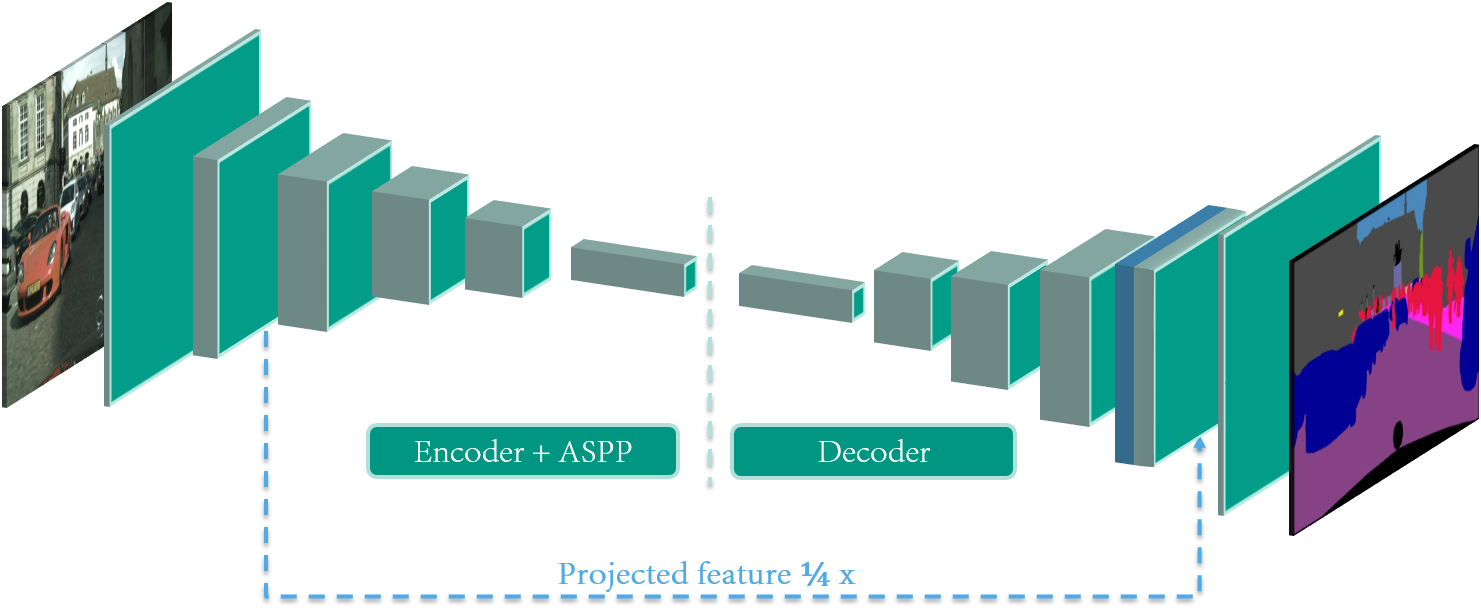
\includegraphics[width = \textwidth]{Graphics/Experimental_Setup/deeplab_image} 
\caption[DeepLab Architecture]{Illustration of DeepLab architecture showing encoder- decoder structure and projected features and atrous spatial pyramid pooling Module (ASPP)}
\label{fig: deeplab_diag} 
\end{figure}

The implemented architecture has been built on top of a deeplab architecture which aims to solve semantic segmentation in an encoder-decoder configuration, where decoder gradually recovers the spatial resolutions by generating output logits equivalent to input image resolution as shown in figure \ref{fig: deeplab_diag}. The panoptic segmentation network extends the deeplab network by an additional decoder branch in addition to the semantic segmentation branch. This newly extended branch is further extended by two heads, where one is responsible for center point predictions and other for offset vector predictions. Each decoder augments its own atrous spatial feature pyramid module that exploit their inherent feature pyramid effect to pool features from latent space independently. Additionally, features from lower layers in encoder are projected to higher layers in both decoders at same spatial resolution i.e. at $1/4$ and $1/8$ of input resolution. These projected features act as skip connections, that feed low-level information from lower layers to higher layers for reconstructing better spatial information. Additionally, during back-propagation parameters from lower layers can exhibit their direct dependency to output logits and can be tuned accordingly. For more details about the implemented architecture, reader is refereed to \cite{Cheng_2020_CVPR}. Another highlight of using such deeplab based semantic segmentation feature extractor is that it exploits a variant of \textit{Xception network} \cite{DBLP:journals/corr/Chollet16a} that is well-suited for learning semantic and pixel-level representations. Adaptations in the xception network and further details about the utilized network architecture have been presented in the figure \ref{fig: modifiedxception}. Further details on how class-agnostic instance segmentation has been achieved is provided in the following chapter.


\begin{figure}[!ht]
\centering 
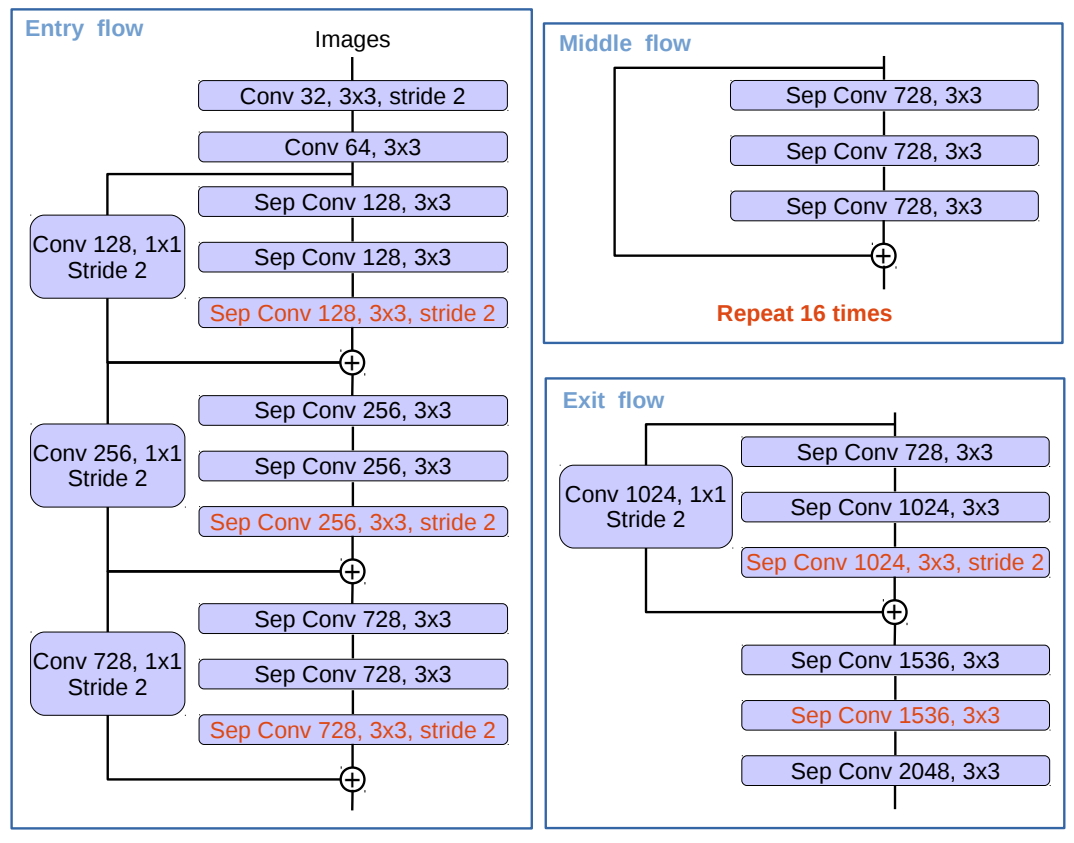
\includegraphics[width = \textwidth]{Graphics/Experimental_Setup/xception} 
\caption[Variant of Xception Architecture]{Figure shows a variant of xception network architecture that is employed in DeepLab feature extractor - showing  (1) more layers in comparison to originally proposed network \cite{DBLP:journals/corr/Chollet16a} (2) max pooling operations are replaced by depth-wise separable convolutions with striding (3) extra batch normalization and ReLU added after each depth-wise convolution. \cite{Deeplabv3+:journals/corr/abs-1802-02611}}
\label{fig: modifiedxception} 
\end{figure}





\bigskip
\begin{sidewaysfigure}
\centering 

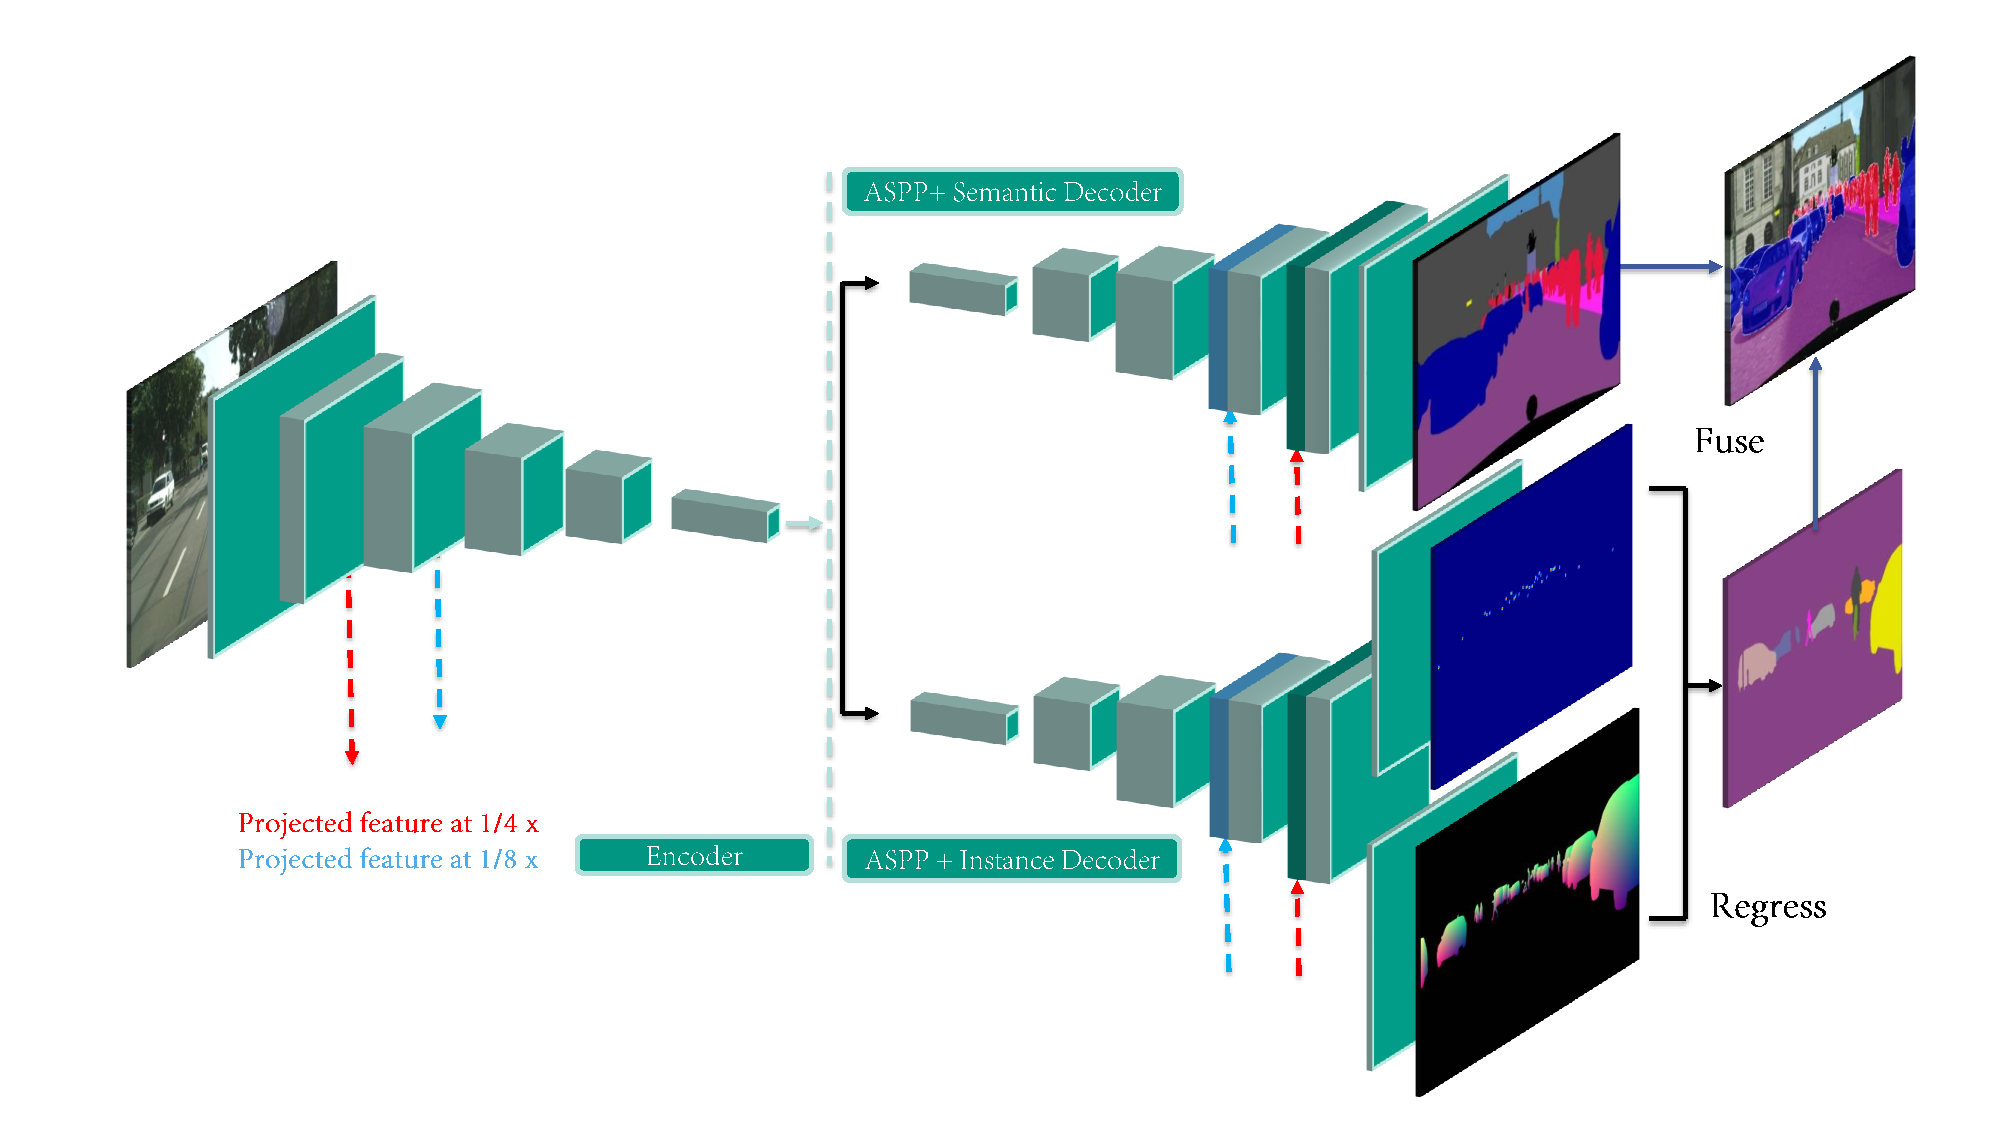
\includegraphics[width = \textwidth]{Graphics/Experimental_Setup/panoptic_deeplab.pdf} 
\caption[Panoptic DeepLab Architecture]{Illustration of Panoptic-DeepLab architecture- showing (1) encoder-decoder structure (2) dual decoder and dual ASPP modules each for semantic decoder and instance decoder (3) projected features at $1/4$ and $1/8$ spatial resolutions (3) instance decoder extended further by two task specific heads for center point predictions and offset vectors prediction.}
\label{fig: panopticdeeplab_diag} 
\end{sidewaysfigure}

\subsection{Semantic Segmentation Head}
Semantic segmentation head as seen in figure \ref{fig: panopticdeeplab_diag} employs \textit{weighted bootstrap cross entropy loss} during training as proposed by \cite{DBLPDeeperLab:journals/corr/abs-1902-05093}. The loss has shown to improve over vanilla bootstrapped cross entropy loss since, each pixel is weighted differently \cite{DBLP:journals/corr/WuSH16b}. Semantic segmentation head is dedicated to learn semantic segmentation of the scene for both \textit{things} and \textit{stuff} classes. 

\subsection{Center Prediction Head}

To learn the center points for instances, groundtruth labels are generated by calculating center of mass for each instance individually followed by an encoding with a standard $2D$ gaussian distribution around each calculated center of mass. To learn such a representation, during training \textit{ Mean Squared Error} (MSE) criterion has been employed to minimize the distance between the predicted heat-map and a groundtruth heat-map \cite{DBLP:journals/corr/TompsonJLB14}. 

\subsection{Offset Prediction Head}

Offset vectors ground-truth labels are generated by calculating distance of each \textit{things} class pixel to its center. By doing so, each pixel encodes distance to it corresponding center in vertical and horizontal direction independently in one channel. $L1$- loss has been employed for training such offset vector representations. During inference, predicted offsets and center points are grouped together to generate class-agnostic instance masks using a simple regression operation.


\section{Evaluation Metrics}


\gls{pq} was the first panoptic segmentation evaluation metric introduced along-with reviving the unified segmentation task \cite{DBLP_panootic_seg:journals/corr/abs-1801-00868}. During evaluation, for each segment a matching is employed that splits the predicted segments in: \gls{tp}, \gls{fp}, \gls{fn} corresponding to matched pairs, unmatched predicted segments and unmatched groundtruth segments. Given the above matching criteria \gls{pq} can be defined as follows:

\begin{equation}\mathrm{PQ}=\frac{\sum_{(p, g) \in T P} \mathrm{IoU}(p, g)}{|T P|+\frac{1}{2}|F P|+\frac{1}{2}|F N|}\end{equation}

\gls{pq} can be seen as a multiplication of two factors:

\begin{equation}\mathrm{PQ}=\frac{\sum_{(p, g) \in T P} \operatorname{IoU}(p, g)}{|T P|} \times \frac{|T P|}{|T P|+\frac{1}{2}|F P|+\frac{1}{2}|F N|}\end{equation}

where the first term has been called \gls{sq} which corresponds to average \gls{iou} of matched segments and second term corresponds to \gls{rq} which is the widely employed F1-score.
However, \gls{pq} treats all segments equally regardless of area i.e.  $10\times10$ and $2000 \times 2000$ pixels are weighted equally \cite{DBLP_panootic_seg:journals/corr/abs-1801-00868}, \cite{DBLPDeeperLab:journals/corr/abs-1902-05093}. 

Therefore, \gls{pc} was recently proposed as an evaluation metric for panoptic segmentation task that remedies the aforementioned problem on equal weighting irrespective of segment size. \gls{pc} can be defined as follows: 

\begin{equation}C o v_{i}=\frac{1}{N_{i}} \sum_{R \in S_{i}}|R| \cdot \max_{R^{\prime} \in S{i}^{\prime}} I O U\left(R, R^{\prime}\right)\end{equation}

\begin{equation}N_{i}=\sum_{R \in S_{i}}|R|\end{equation}

\begin{equation}P C=\frac{1}{C} \sum_{i=1}^{C} C o v_{i}\end{equation}

where $S_{i}$ and $S_{i}^{\prime}$ are groundtruth and predicted segments of given class $i$, and $N_{i}$ is the number of pixels in groundtruth region. \gls{pc} can be calculated by computing the average of $Cov_{i}$ over $C$ number of semantic classes. Reader is refereed to \cite{DBLPDeeperLab:journals/corr/abs-1902-05093} for further information on evaluation metric. 

For evaluation purposes, \gls{pc} has been chosen to report and document evaluation and comparison of experiments for presented work.

\section{Hyper-parameter Specifications}

This section specifies hyper-parameters used in experiments carried out during the scope of this work. Since, a suitable hyper-parameter configuration is critical for efficient training, most of the below mentioned hyper-parameters were chosen based on best practices in the literature and were defined at an early stage of this work.  Hyper-parameter manipulation among the experiments is kept to a minimum to ensure comparability and meaningful evaluation of the results. However some parameters used in post-processing and did not have an effect on training process were chosen after extensive evaluation to squeeze best performance.

Additionally, due to limited computational resources, two stage training process has been adapted, where first stage has relatively larger batch size with smaller image crops to enable focus on smaller details and make use multiple samples in each step. To learn a holistic scene representation, a larger crop size is adapted while sacrificing on batch size in the subsequent stage. 


\paragraph{Learning Rate}

For a learning process, learning rate defines how fast the network weights are adapted with respect to gradient in a single optimisation step. See section \ref{subsec:learningnopt} for more details. A higher learning rate results in faster adaptation of weights, however it might result in a sub-optimal solution. Usually, a very small learning rate is adapted to slowly converge towards an optimal solution whilst avoiding local-minimum. Learning rate for all the experiments carried out during presented work is chosen to be $0.001$.

\paragraph{Batch Size}

Batch size defines the number of samples chosen for each step during a learning process. The network parameters are optimised during each iteration with respect to number of samples at hand, defined by batch size parameter. Usually, a relatively higher batch size is preferred to include diversity and make use of GPU parallelism to speed up learning process. In the first stage a batch size of $4$ is chosen, while in the second stage batch size is chosen to be $1$.

\paragraph{Input Shape}

All the input images that are passed through the network are expected to be of same input resolution. Deeplab architecture adapts to various input resolutions. In the first stage of training process, input images are cropped to $769\times769$ resolution, whereas, in the second stage input images are cropped to $1025\times1025$ spatial resolution.

\paragraph{Number of iterations}

Number of update steps in a training process are defined by number of iterations. In the presented work, training is carried out in two stages. For the first stage, number of iterations are set to be $150,000$ while in the second stage (with larger crop size and single batch size) number of iterations are set to be $50,000$.

\paragraph{Optimizer}

To ensure compatibility and standardized comparison, all the reported experiments carried out during the course of presented work employed \textit{Adam} as an optimizer \cite{Goodfellow-et-al-2016} with \textit{poly learning rate decay}. See section \ref{subsec:learningnopt} for more details.  


\paragraph{Regularization}

To avoid over-fitting and improve generalization presented work uses batch normalization, dropout and weight decay for regularization purposes. 

\paragraph{Number of project features}

As mentioned in the previous section of this chapter, the network makes use of low-level features by sharing information between encoder and decoder modules i.e. low-level features from encoder (at spatial resolution $1/4$ and $1/8$ of original input size) are projected at the same spatial resolution in both decoders independently, as shown in the figure \ref{fig: panopticdeeplab_diag}. Before concatenating with decoder features the projected features are passed through a convolution operation to reduce number of channels (by a point-wise convolution) see section \ref{subsec:atroussepconv}, which defines the number of projected features. Number of projected features for semantic decoder are fixed to $32$ and $64$ at spatial resolution $1/4$ and $1/8$ of input size respectively. While, number of projected features for instance decoder are set $16$ and $32$ at spatial resolution $1/4$ and $1/8$ of input size respectively.


\paragraph{Center Pooling Kernel Size}

The network predicts a probability distribution around each center point, however it is desired to extract exact locations for each center prediction. To this end, max pooling is employed that only keeps the pixel location with maximum prediction confidence each kernel window. The size of this pooling kernel can be adapted. Since this is a post-processing step and does not influence learning, various kernel window sizes have been compared against each other and kernel window of $72\times72$ was observed to yield best results and was fixed for further experimental evaluations.

\paragraph{Number of Instances}

Another parameter that is part of post-processing step and does not affect learning process is the number of instances. After pooling the center points using a fixed kernel window, the number of filtered center points are limited by selecting top 200 centers according to their prediction confidence. 

\paragraph{Deep Learning Framework}

To implement bottom-up panoptic segmentation network architecture and to carry out experiments \textit{Tensorflow framework} has been used since it is highly flexible regarding implementation and provides extensive documentation. In addition, it provides an integrated tool called \textit{Tensorboard} that enables online monitoring and comparison between experiments. Therefore, network architecture implementation and conduction of experiments was carried out using Tensorflow framework.  





